\documentclass{article}
\usepackage{amsmath}
\usepackage{graphicx}

\begin{document}
	
	\section*{Hamiltonianos do Sistema Sierpinski}
	

	\section*{Ensemble $\mathbf{\beta=1}$}
	\begin{equation}
		H=\sum_{i\in \text{Sierpinski}}\epsilon_{i}c_{i}^{\dagger}c_{i}-\sum_{\langle i,j\rangle\in \text{Sierpinski}}tc_{i}^{\dagger}c_{j}
	\end{equation}
	

	\section*{Ensemble $\mathbf{\beta=2}$}
	\begin{equation}
		H=\sum_{i\in \text{Sierpinski}}\epsilon_{i}c_{i}^{\dagger}c_{i}-\sum_{\langle i,j\rangle\in \text{Sierpinski}}t_{ij}c_{i}^{\dagger}c_{j}
	\end{equation}
	
	$t_{ij}=\sigma_{0}e^{i\frac{\phi}{2}(x_{i}-x_{j})(y_{i}+y_{j})}$
	

	\section*{Ensemble $\mathbf{\beta=4}$}
	\begin{equation}
		H=\sum_{i\in \text{Sierpinski}}(\epsilon_{i}+e_{z}\sigma_{z})c_{i}^{\dagger}c_{i}-\sum_{\langle i,j\rangle_{x}}(t\sigma_{0}-\frac{i\alpha}{2}\sigma_{y})c_{i}^{\dagger}c_{j}-\sum_{\langle i,j\rangle_{y}}(t\sigma_{0}+\frac{i\alpha}{2}\sigma_{x})c_{i}^{\dagger}c_{j}
	\end{equation}
	
	\vspace*{1cm}
	
	\section*{Informação sobre o cálculo da dimensão fractal}
	
	Na figura abaixo, transladamos verticalmente todas os pontos e a reta de modo que o primeiro ponto de cada reta coincida com a origem. Dado que a dimensão fractal é dada pelo valor do coeficiente angular, este procedimento não altera o resultado da dimensão fractal. 
	
	Com isso é possível mostrar claramente que a inclinação da reta aumenta com $m$, em outras palavras, quanto maior a ordem $m$ do fractal, maior a dimensão fractal das curvas de condutância e ruído de disparo. Em $m=0$, o valor da dimensão fractal calculada pelo método box-counting converge para o valor da Dimensão de Hausdorff do carpete de sierpinski.
	
	\begin{table}[h!]
		\centering
		\begin{tabular}{c|ccccc}
			\hline
			& $m=0$ & $m=1$ & $m=2$ & $m=3$ & $m=4$ \\
			\hline
			$\beta = 1$ (G) & 1.69 & 1.79 & 1.85 & 1.86 & 1.88 \\
			$\beta = 2$ (G) & 1.33 & 1.62 & 1.73 & 1.81 & 1.86 \\
			$\beta = 4$ (G) & 1.19 & 1.44 & 1.75 & 1.80 & 1.86 \\
			$\beta = 1$ (P) & 1.69 & 1.73 & 1.78 & 1.81 & 1.88 \\
			$\beta = 2$ (P) & 1.45 & 1.67 & 1.73 & 1.65 & 1.85 \\
			$\beta = 4$ (P) & 1.23 & 1.37 & 1.60 & 1.83 & 1.87 \\
			\hline
		\end{tabular}
		\caption{Dimensão fractal.}
		\label{tab:beta_m}
	\end{table}
	
	
	
	\begin{figure}[htbp]  % h=here, t=top, b=bottom, p=page
		\centering
		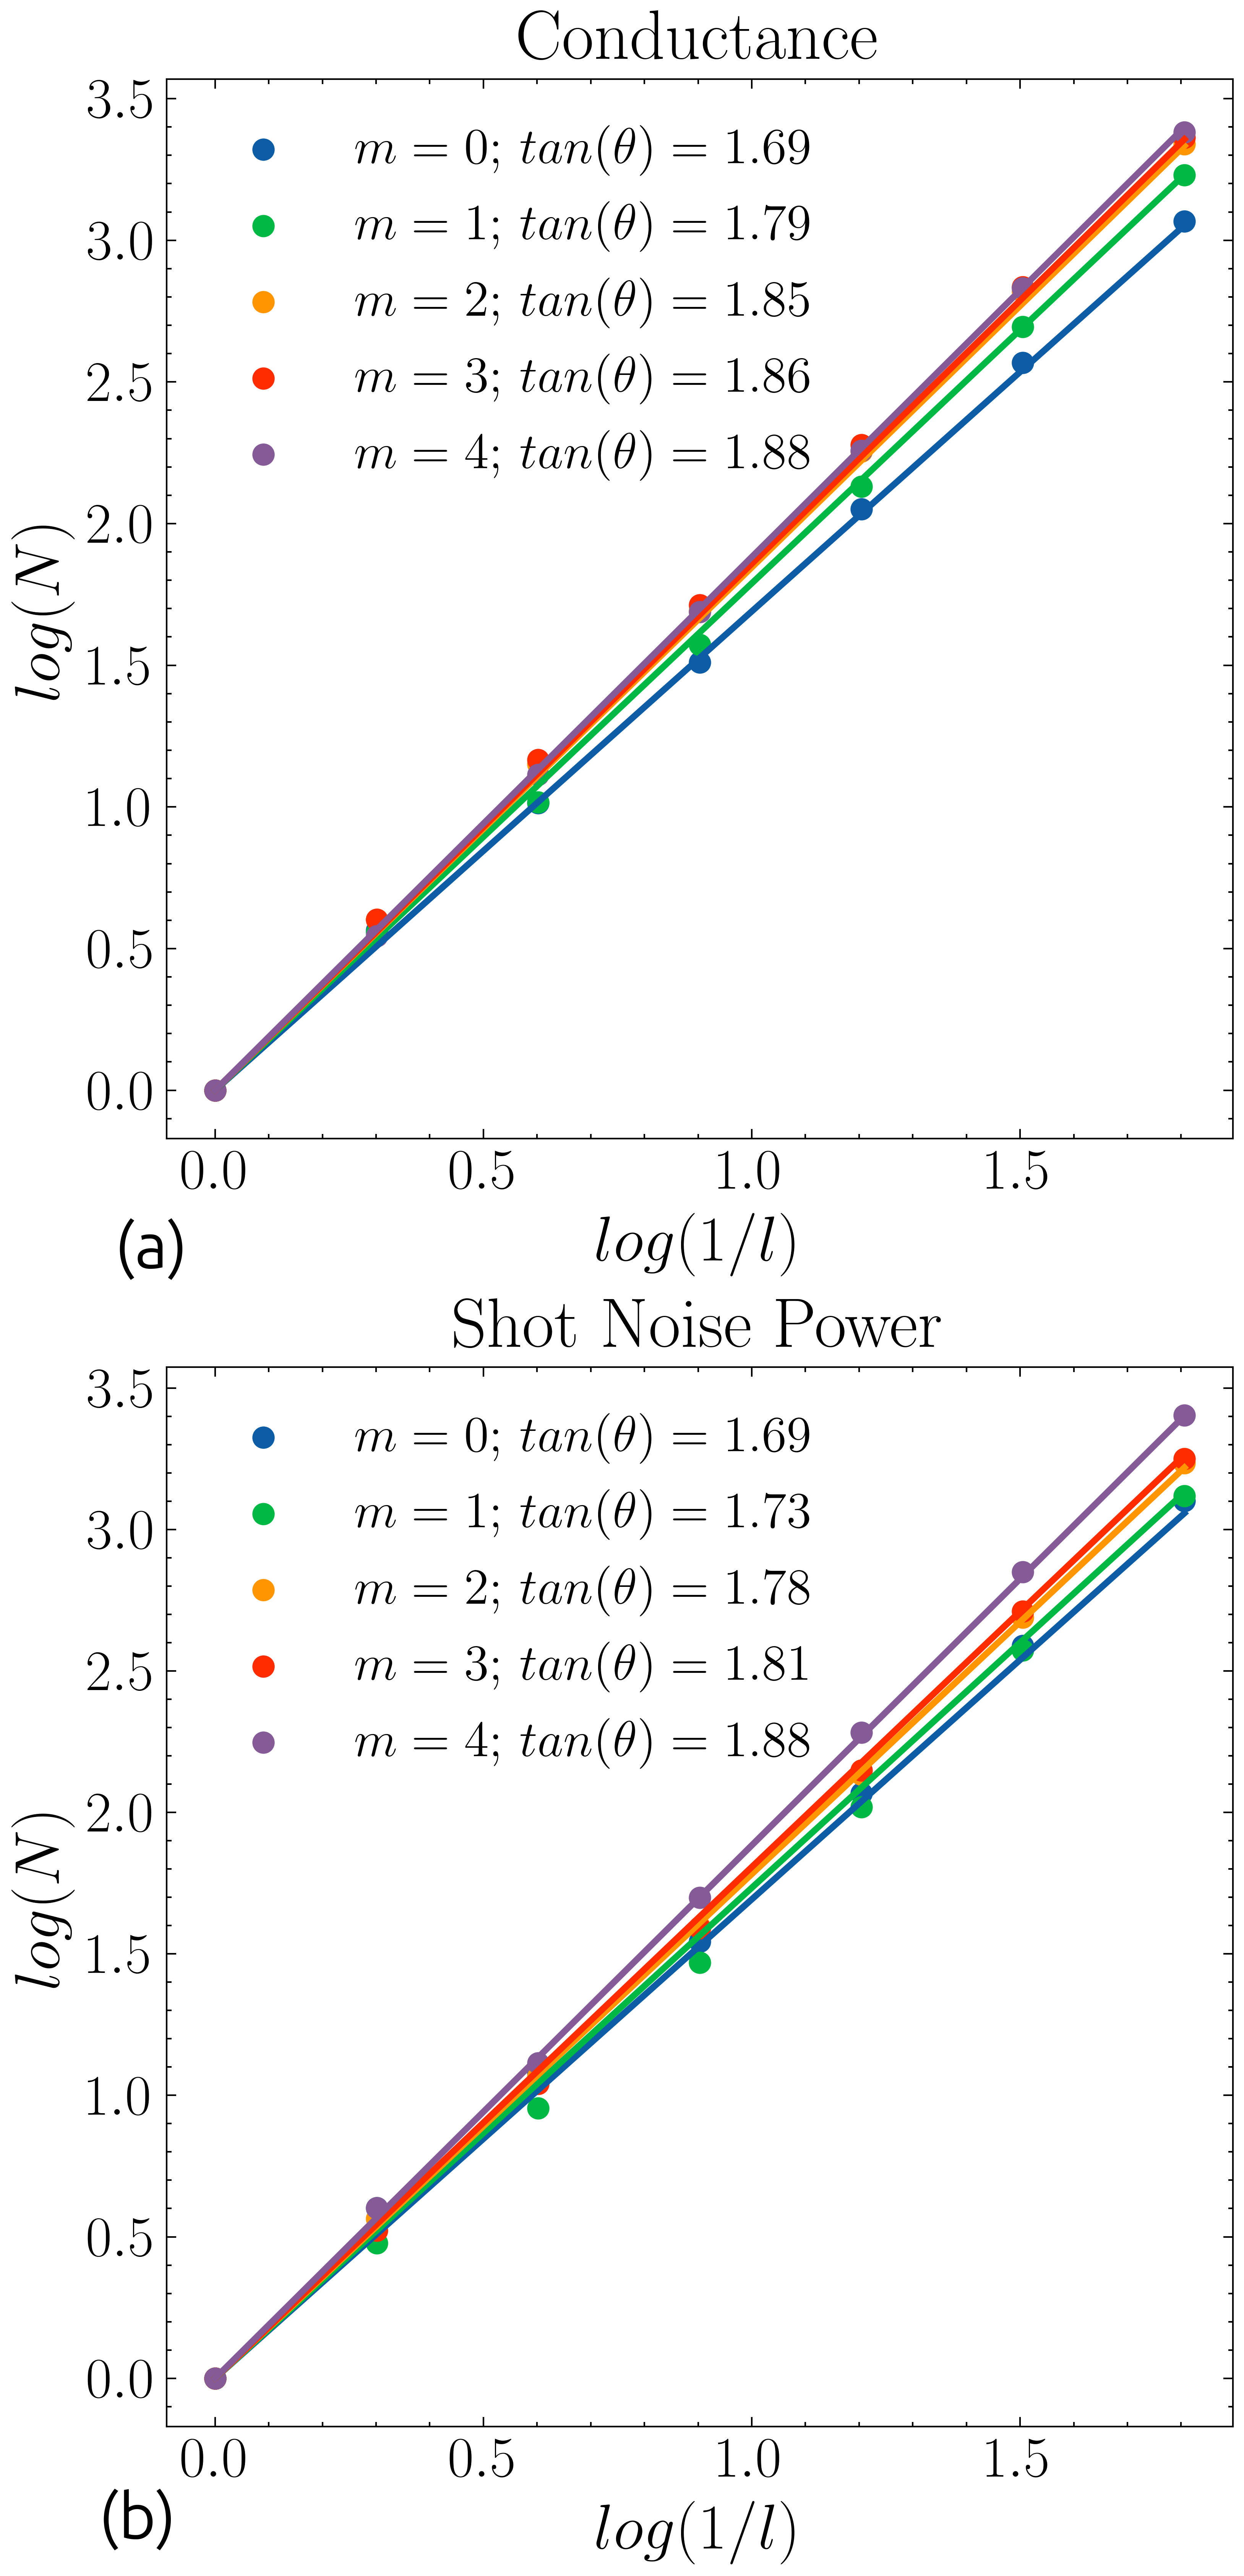
\includegraphics[width=0.6\textwidth]{fig5.png}
		\caption{Legenda da imagem}
		\label{fig:minha_imagem}
	\end{figure}
	
	
\end{document}